\section*{Fresh peer messages changed predictions}
\begin{center}
\begin{tabular}{rrrrrrr}
\toprule
Seed & Fresh & Static & Gained & Lost & Stale clamp & Serial reader\\
\midrule
31 & 351 & 344 & 22 & 15 & 198 & 251\\
47 & 358 & 357 & 9 & 8 & 198 & 277\\
83 & 340 & 362 & 4 & 26 & 152 & 368\\
\bottomrule
\end{tabular}
\end{center}
Counts are correct queries out of the same 368. Gained and lost compare separately trained fresh and static models on paired inputs. The mean fresh-minus-static difference was $-1.27$ percentage points. The 95\% interval from 2,000 draws of 92 operation pairs was $[-2.81,+0.27]$ points conditional on the three training seeds. All six dense models fit training exactly; none triggered the extension. Static reached 96.29\%, leaving less than the registered five-point margin even for a perfect challenger. The identity-second-table control had fresh/static scores of 16/15, 16/16 and 15/16 out of 16.
\par
\textbf{One changed prediction.} For seed 31, query 2, $F=(2,1,0,3)$ and $G=(0,3,1,2)$, the correct answer was 0. The fresh model returned 1. Both clamping and the separately trained static model returned 0. Conversely, one fresh-only gain survived clamping. Intervening on a learned wire and retraining without the wire answer different questions.
\par
\textbf{What the donor could transmit.} For each seed, 100 inputs had matched eligible donors. Active message transplants produced the donor target 39, 44 and 53 times; placebo transplants preserved the original prediction 93, 92 and 89 times. With $G,q$ fixed and $G$ bijective, the correct intermediate uniquely identifies the final answer and vice versa. This design cannot distinguish a message carrying $F(q)$ from one carrying $G(F(q))$.
\par
\textbf{Optimization and cost.} A 20-parameter two-read model acquired the intended table order in all seeds. Only seed 83 acquired the identity address map and solved all queries. The other two suppressed the correct address and reached 251 and 277. The deterministic table follower solved every case. These results distinguish an available algorithm from its reliable acquisition. Both dense arms used 4,708 parameters and 10,752 dense multiply-accumulates per query. The serial reader used 112 multiplications in its matrix reads and mixtures. Latencies include framework dispatch. PH1 used NumPy, the reader used PyTorch; neither implementation sets a hardware lower bound.
\par
\begin{center}
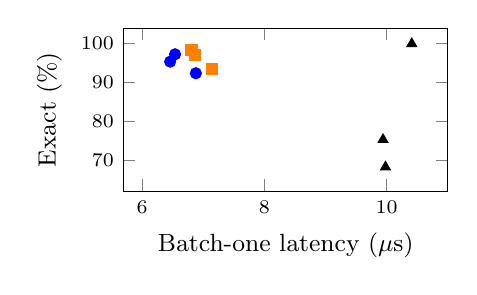
\begin{tikzpicture}
\begin{axis}[width=.47\linewidth,height=3.65cm,xlabel={Batch-one latency ($\mu$s)},ylabel={Exact (\%)},xmin=5.7,xmax=11,ymin=62,ymax=104,tick label style={font=\scriptsize},label style={font=\small}]
\addplot[only marks,mark=*,blue] coordinates {(6.46,95.38)(6.54,97.28)(6.88,92.39)};
\addplot[only marks,mark=square*,orange] coordinates {(7.14,93.48)(6.87,97.01)(6.81,98.37)};
\addplot[only marks,mark=triangle*,black] coordinates {(9.98,68.21)(9.94,75.27)(10.41,100)};
\end{axis}
\end{tikzpicture}
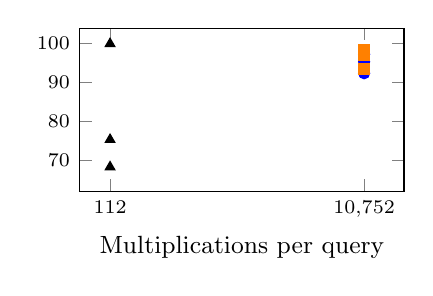
\begin{tikzpicture}
\begin{semilogxaxis}[width=.47\linewidth,height=3.65cm,xlabel={Multiplications per query},xmin=65,xmax=22000,ymin=62,ymax=104,xtick={112,10752},xticklabels={112,{10,752}},tick label style={font=\scriptsize},label style={font=\small}]
\addplot[only marks,mark=*,blue] coordinates {(10752,95.38)(10752,97.28)(10752,92.39)};
\addplot[only marks,mark=square*,orange] coordinates {(10752,93.48)(10752,97.01)(10752,98.37)};
\addplot[only marks,mark=triangle*,black] coordinates {(112,68.21)(112,75.27)(112,100)};
\end{semilogxaxis}
\end{tikzpicture}\\[-2pt]
{\small Circles: fresh. Squares: static. Triangles: serial. Each point is one seed.}
\end{center}
